\section{Osnovna kombinatorična načela}
Če želimo prešteti neke objekte s predpisanimi lastnostmi, to lahko storimo v dveh delih:
\begin{itemize}
    \item najprej objekte ki jih preštevamo, združimo jih v neko natančno opisano množico
    \item nato pa tej množici določimo moč
\end{itemize}

\subsection{Definicija}
Pravimo da končna množica $X$ \underline{vsebuje $n$ elementov}, če obstaja bijekcija iz množice $X$ v množico $\{1, 2, 3, \dots, n\}$. U tem primeru pištemo $|X|=n$ in rečemo da je \underline{moč} množice $X$ enaka $n$. Prazno množico obravnavamo posebej in postavimo $|\emptyset|= 0$. \\[1em]
Pri določanju moči množice si pomagamo z nekaj preprostimi načeli.

\subsection{Izrek (načelo vsote)}
Če sta $A$ in $B$ končni disjunktni množici potem velja $|A \cup B| = |A| + |B|$.
S pomočjo matematične indukcije načelo vsote posplošimo na končno unijo paroma disjunktnih končnih množic.
Če so $A_1, A_2, \dots, A_n$ končne in paroma disjunktne množice (tj. $A_i \cap A_j = \emptyset$ za $i \ne j$), potem velja naslednje:
\begin{align*}
    |A_1 \cup A_2 \cup \dots \cup A_n| = |A_1| + |A_2| + \dots + |A_n|    
\end{align*}
oziroma:
\begin{align*}
    \left| \bigcup_{i = 1}^n A_i \right| = \sum_{i = 1}^n |A_i|
\end{align*}


\subsection{Zgled}
Od mesta $X$ do mesta $Y$ lahko pridemo z letalom, vlakom ali avtobusom. Med $X$ in $Y$ je 12 različnih letalskih poletov, 5 različnih vlakov in 10 različnih avtobusov. Koliko različnih množic imamo, da pridemo iz $X$ v $Y$? \\[1em]
Izberemo lahko le en način prevoza. 
In za vsak način imamo izbiro: $12 + 5 + 10 = 27$


\subsection{Izrek (načelo enakosti)}
Če obstaja bijekcija med dvema končnima množicama $A$ in $B$, potem je $|A| = |B|$.


\subsection{Zgled}
Naj bo $X$ množica z $n$ elementi, koliko podmnožic premore $X$?
\begin{align*}
    X = \{x_1, x_2, & x_3\} \text{ } \text{ } \text{ } 8 = 2^3 \\[1em]
    \emptyset & \to (0,0,0) \\
    \{x_1\} & \to (1,0,0) \\
    \{x_2\} & \to (0,1,0) \\
    \{x_3\} & \to (0,0,1) \\
    \{x_1,x_2\} & \to (1,1,0) \\
    \{x_1,x_3\} & \to (1,0,1) \\
    \{x_2,x_3\} & \to (0,1,1) \\
    \{x_1,x_2,x_3\} & \to (1,1,1) \\[1em]
    P(\{x_1,x_2,x_3\}) = \{
        \emptyset, \{x_1\}, \{x_2\}, \{x_3\}, & \{x_1,x_2\}, \{x_1,x_3\}, \{x_2,x_3\}, \{x_1,x_2,x_3\}
    \}
\end{align*}
Naloga sprašuje po moči potenčne množice $P(X)$ množice $X$. ($2^X$)
Rešimo jo tako da poiščemo bijekcijo med množico $P(X)$ in množico vseh narejenih n-teric z elementi iz množice $\{0, 1\}$.
Označimo elemente množice $X$ z $x_1, x_2, \dots, x_n$. Poljubni množici $Y \in P(X)$ priredimo $\chi(Y) = (y_1, y_2, \dots, y_n) \in \{0, 1\}^n$ za katerega je
$$
y_i = 
\begin{cases}
    1; & \text{če } x_i \in Y \\
    0; & \text{sicer } \\
\end{cases}
$$  
Na ta način smo definirali preslikavo 
$$
\chi : P(X) \to \{0, 1\}^n
$$
Ta preslikava je bijektivna. Zato je
$$
|P(X)| = |\{0, 1\}^n| = 2^n
$$




\subsection{Načelo dvojnega preštevanja}
Če isto množico preštejemo na dva različna načina, potem sta odgovora enaka.
Učasih se imenuje tudi "računovodsko načelo".
Načelo je analogno iskanju vsote vseh elentov v matriki tako, da seštejete vsote vseh vrstic, nato pa raun preverite tako da seštejete vsoto stolpcev.
\begin{figure}[H]
    \centering



\tikzset{every picture/.style={line width=0.75pt}} %set default line width to 0.75pt        

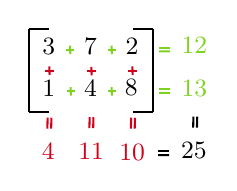
\begin{tikzpicture}[x=0.75pt,y=0.75pt,yscale=-1,xscale=1]
%uncomment if require: \path (0,300); %set diagram left start at 0, and has height of 300

%Straight Lines [id:da9876418121717137] 
\draw    (100.11,79.96) -- (100.11,120.21) ;
%Straight Lines [id:da9982003751714028] 
\draw    (160.11,79.96) -- (160.11,120.21) ;
%Straight Lines [id:da8853245130637188] 
\draw    (109.86,120.21) -- (100.11,120.21) ;
%Straight Lines [id:da6977665563462152] 
\draw    (109.86,79.96) -- (100.11,79.96) ;
%Straight Lines [id:da19611108214265327] 
\draw    (160.11,79.96) -- (150.36,79.96) ;
%Straight Lines [id:da42792423343183295] 
\draw    (160.11,120.21) -- (150.36,120.21) ;
%Straight Lines [id:da6058115450979873] 
\draw [color={rgb, 255:red, 208; green, 2; blue, 27 }  ,draw opacity=1 ]   (110.06,98.11) -- (110.16,102.21) ;
%Straight Lines [id:da8772001572095638] 
\draw [color={rgb, 255:red, 208; green, 2; blue, 27 }  ,draw opacity=1 ]   (112.11,100.19) -- (108.11,100.19) ;
%Straight Lines [id:da8340591451035007] 
\draw [color={rgb, 255:red, 208; green, 2; blue, 27 }  ,draw opacity=1 ]   (130.31,98.36) -- (130.41,102.46) ;
%Straight Lines [id:da29212752045444] 
\draw [color={rgb, 255:red, 208; green, 2; blue, 27 }  ,draw opacity=1 ]   (132.36,100.44) -- (128.36,100.44) ;
%Straight Lines [id:da3192937194200052] 
\draw [color={rgb, 255:red, 208; green, 2; blue, 27 }  ,draw opacity=1 ]   (150.06,98.11) -- (150.16,102.21) ;
%Straight Lines [id:da9297025364071232] 
\draw [color={rgb, 255:red, 208; green, 2; blue, 27 }  ,draw opacity=1 ]   (152.11,100.19) -- (148.11,100.19) ;
%Straight Lines [id:da41217905607586847] 
\draw [color={rgb, 255:red, 126; green, 211; blue, 33 }  ,draw opacity=1 ]   (120.06,88.11) -- (120.16,92.21) ;
%Straight Lines [id:da988514893130142] 
\draw [color={rgb, 255:red, 126; green, 211; blue, 33 }  ,draw opacity=1 ]   (122.11,90.19) -- (118.11,90.19) ;
%Straight Lines [id:da972167095048927] 
\draw [color={rgb, 255:red, 126; green, 211; blue, 33 }  ,draw opacity=1 ]   (120.31,108.11) -- (120.41,112.21) ;
%Straight Lines [id:da5905123219537465] 
\draw [color={rgb, 255:red, 126; green, 211; blue, 33 }  ,draw opacity=1 ]   (122.36,110.19) -- (118.36,110.19) ;
%Straight Lines [id:da16654630461039455] 
\draw [color={rgb, 255:red, 126; green, 211; blue, 33 }  ,draw opacity=1 ]   (140.06,108.11) -- (140.16,112.21) ;
%Straight Lines [id:da7079509735983525] 
\draw [color={rgb, 255:red, 126; green, 211; blue, 33 }  ,draw opacity=1 ]   (142.11,110.19) -- (138.11,110.19) ;
%Straight Lines [id:da5061884093026838] 
\draw [color={rgb, 255:red, 126; green, 211; blue, 33 }  ,draw opacity=1 ]   (140.06,88.11) -- (140.16,92.21) ;
%Straight Lines [id:da014846693565639058] 
\draw [color={rgb, 255:red, 126; green, 211; blue, 33 }  ,draw opacity=1 ]   (142.11,90.19) -- (138.11,90.19) ;
%Straight Lines [id:da06036658099407499] 
\draw [color={rgb, 255:red, 126; green, 211; blue, 33 }  ,draw opacity=1 ]   (168.2,90.88) -- (162.95,90.89) ;
%Straight Lines [id:da7598309739737914] 
\draw [color={rgb, 255:red, 126; green, 211; blue, 33 }  ,draw opacity=1 ]   (168.19,89.05) -- (162.94,89.05) ;
%Straight Lines [id:da5077711648266361] 
\draw [color={rgb, 255:red, 126; green, 211; blue, 33 }  ,draw opacity=1 ]   (168.2,110.88) -- (162.95,110.89) ;
%Straight Lines [id:da2621406983997041] 
\draw [color={rgb, 255:red, 126; green, 211; blue, 33 }  ,draw opacity=1 ]   (168.19,109.05) -- (162.94,109.05) ;
%Straight Lines [id:da7279670099670634] 
\draw [color={rgb, 255:red, 208; green, 2; blue, 27 }  ,draw opacity=1 ]   (109.09,128.07) -- (109.22,122.82) ;
%Straight Lines [id:da9642997740936594] 
\draw [color={rgb, 255:red, 208; green, 2; blue, 27 }  ,draw opacity=1 ]   (110.92,128.11) -- (111.05,122.86) ;
%Straight Lines [id:da0748947581710866] 
\draw [color={rgb, 255:red, 208; green, 2; blue, 27 }  ,draw opacity=1 ]   (129.34,127.82) -- (129.47,122.57) ;
%Straight Lines [id:da4708834491306948] 
\draw [color={rgb, 255:red, 208; green, 2; blue, 27 }  ,draw opacity=1 ]   (131.17,127.86) -- (131.3,122.61) ;
%Straight Lines [id:da5861063707955871] 
\draw [color={rgb, 255:red, 208; green, 2; blue, 27 }  ,draw opacity=1 ]   (149.34,128.07) -- (149.47,122.82) ;
%Straight Lines [id:da130817506793925] 
\draw [color={rgb, 255:red, 208; green, 2; blue, 27 }  ,draw opacity=1 ]   (151.17,128.11) -- (151.3,122.86) ;
%Straight Lines [id:da7686233956600592] 
\draw [color={rgb, 255:red, 0; green, 0; blue, 0 }  ,draw opacity=1 ]   (179.34,127.57) -- (179.47,122.32) ;
%Straight Lines [id:da22623864842508312] 
\draw [color={rgb, 255:red, 0; green, 0; blue, 0 }  ,draw opacity=1 ]   (181.17,127.61) -- (181.3,122.36) ;
%Straight Lines [id:da6297533413950192] 
\draw [color={rgb, 255:red, 0; green, 0; blue, 0 }  ,draw opacity=1 ]   (167.7,140.88) -- (162.45,140.89) ;
%Straight Lines [id:da3714418029236315] 
\draw [color={rgb, 255:red, 0; green, 0; blue, 0 }  ,draw opacity=1 ]   (167.69,139.05) -- (162.44,139.05) ;

% Text Node
\draw (105.25,83.15) node [anchor=north west][inner sep=0.75pt]  [font=\small] [align=left] {3};
% Text Node
\draw (125.25,83.15) node [anchor=north west][inner sep=0.75pt]  [font=\small] [align=left] {7};
% Text Node
\draw (125.25,103.15) node [anchor=north west][inner sep=0.75pt]  [font=\small] [align=left] {4};
% Text Node
\draw (145,102.9) node [anchor=north west][inner sep=0.75pt]  [font=\small] [align=left] {8};
% Text Node
\draw (105.25,103.15) node [anchor=north west][inner sep=0.75pt]  [font=\small] [align=left] {1};
% Text Node
\draw (145.25,83.15) node [anchor=north west][inner sep=0.75pt]  [font=\small] [align=left] {2};
% Text Node
\draw (105,133.65) node [anchor=north west][inner sep=0.75pt]  [font=\small] [align=left] {\textcolor[rgb]{0.82,0.01,0.11}{4}};
% Text Node
\draw (122.5,133.65) node [anchor=north west][inner sep=0.75pt]  [font=\small,color={rgb, 255:red, 208; green, 2; blue, 27 }  ,opacity=1 ] [align=left] {11};
% Text Node
\draw (142.25,134.15) node [anchor=north west][inner sep=0.75pt]  [font=\small,color={rgb, 255:red, 208; green, 2; blue, 27 }  ,opacity=1 ] [align=left] {10};
% Text Node
\draw (172.25,82.9) node [anchor=north west][inner sep=0.75pt]  [font=\small,color={rgb, 255:red, 126; green, 211; blue, 33 }  ,opacity=1 ] [align=left] {12};
% Text Node
\draw (172.25,103.15) node [anchor=north west][inner sep=0.75pt]  [font=\small,color={rgb, 255:red, 126; green, 211; blue, 33 }  ,opacity=1 ] [align=left] {13};
% Text Node
\draw (172,133.15) node [anchor=north west][inner sep=0.75pt]  [font=\small,color={rgb, 255:red, 0; green, 0; blue, 0 }  ,opacity=1 ] [align=left] {25};


\end{tikzpicture}
    
\end{figure}

\subsection{Zgled (uporabe načela dvojnega preštevanja)}

\subsubsection{Lema (lema o rokovanju)}
Na kongresu je število vseh vdeležencev ki se rokojejo liho mnogokrat, sodo.
\begin{figure}[H]
    \centering

    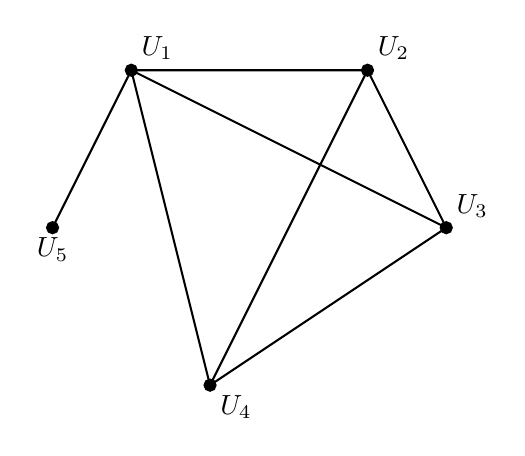
\begin{tikzpicture}
        
        % Points
        \draw[fill=black] (1,1) circle (2pt) node[below] {$U_5$};
        \draw[fill=black] (2,3) circle (2pt) node[above right] {$U_1$};
        \draw[fill=black] (5,3) circle (2pt) node[above right] {$U_2$};
        \draw[fill=black] (6,1) circle (2pt) node[above right] {$U_3$};
        \draw[fill=black] (3,-1) circle (2pt) node[below right] {$U_4$};

        
        % Lines
        \draw (1,1) -- (2,3) -- (5,3) -- (6,1) -- (3, -1) -- (2, 3);
        \draw (6,1) -- (2,3);
        \draw (3, -1) -- (5, 3);
    \end{tikzpicture}
    
\end{figure}

\begin{align*}
    % some math here
    U_1&: U_2, U_3, U_4, U_5 & x_1 = 4 && y = 7 \text{ }(\text{skupno število rokovanj})\\ 
    U_2&: U_1, U_3, U_4      & x_2 = 3 \\
    U_3&: U_2, U_1, U_4      & x_3 = 3 \\
    U_4&: U_1, U_2, U_3      & x_4 = 3 \\
    U_5&: U_1                & x_5 = 1 \\
\end{align*}


\subsubsection{Dokaz}
Naj bodo od $U_1, \dots, U_n$ udeleženci kongresa. Načelo dvojnega preštevanja bomo uporabili na množici urejenih parov $(U_1, U_j)$, za katere se udeleženca $U_i$ in $U_j$ rokojeta. Naj bo $x_i$ število udeležencev s katerimi se je $U_i$ rokoval in $y$ skupno število rokovanj.
Po eni strani je to število parov enako:
\begin{align*}
    \sum_{i = 1}^{n} x_i
\end{align*}
saj je za vsak $U_i$ število izbir enako $x_i$. Po drugi strani pa vsako rokovanje poredi natanko dva para:
\begin{align*}
    (U_i, U_j) \text{ in } (U_j, U_i)
\end{align*}
skupno število parov je tako $2y$.
Torej velja:
\begin{align*}
    \sum_{i = 1}^{n} x_i & = 2y \\
    4 + 3 + 3 + & 3 + 1 = 14 
\end{align*}
Če pa je vsota $n$ celih števil sodo število lihih sumandov sodo.
Načelo se navadno uporablja za štetje urejenih parov.


\subsubsection{Izrek}
Naj bosta $A = \{ a_1, \dots, a_m \}$ in $B = \{ b_1, \dots, b_n \}$ množici in naj bo $S \subseteq A \times B$. \\
Naj bo za vse $i = 1, \dots, n$ element $a_i$ prva koordinata $x_i$ parov množice $S$, medtem ko je za vse $j = 1, \dots, n$ element $b_j$ druga koordinata $y_j$ parov množice $S$. Tedaj velja:
\begin{align*}
    |S| = \sum_{i = 1}^{m} x_i = \sum_{j = 1}^{n} y_j    
\end{align*}


\subsubsection{Zgled}
\begin{align*}
    & A = \{ 1, 2, 3 \} \text{ } B = \{u, v\} \\[1em]
    & A \times B = \{ (1, u), (1, v), (2, u), (2, v), (3, u), (3,v) \} \\[1em]
    & S = \{ (1, u), (1, v), (2, u), (3, v) \}
\end{align*}
\begin{figure}[H]
    \centering



\tikzset{every picture/.style={line width=0.75pt}} %set default line width to 0.75pt        

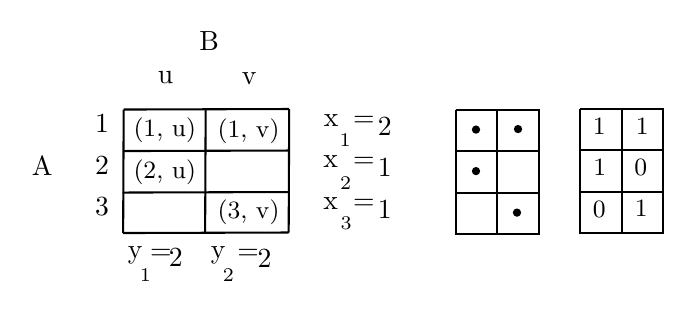
\begin{tikzpicture}[x=0.75pt,y=0.75pt,yscale=-1,xscale=1]
%uncomment if require: \path (0,300); %set diagram left start at 0, and has height of 300

%Straight Lines [id:da5837397187437077] 
\draw    (100.35,80.44) -- (100.1,139.94) ;
%Straight Lines [id:da07408006488012053] 
\draw    (180.1,80.19) -- (179.85,139.69) ;
%Straight Lines [id:da3018521643649703] 
\draw    (139.85,80.19) -- (139.6,139.69) ;
%Straight Lines [id:da8678587668039301] 
\draw    (100.1,139.94) -- (179.85,139.69) ;
%Straight Lines [id:da0008770237972171024] 
\draw    (180.1,80.19) -- (100.35,80.44) ;
%Straight Lines [id:da04709743516442333] 
\draw    (180.35,100.19) -- (100.6,100.44) ;
%Straight Lines [id:da13675277449821688] 
\draw    (179.6,120.19) -- (99.85,120.44) ;
%Shape: Grid [id:dp6093691984108132] 
\draw  [draw opacity=0] (260.25,80.5) -- (300.85,80.5) -- (300.85,141.1) -- (260.25,141.1) -- cycle ; \draw   (260.25,80.5) -- (260.25,141.1)(280.25,80.5) -- (280.25,141.1)(300.25,80.5) -- (300.25,141.1) ; \draw   (260.25,80.5) -- (300.85,80.5)(260.25,100.5) -- (300.85,100.5)(260.25,120.5) -- (300.85,120.5)(260.25,140.5) -- (300.85,140.5) ; \draw    ;
%Shape: Free Drawing [id:dp00586274156487554] 
\draw  [line width=3] [line join = round][line cap = round] (270.1,90.1) .. controls (270.1,90.1) and (270.1,90.1) .. (270.1,90.1) ;
%Shape: Free Drawing [id:dp6928199422489496] 
\draw  [line width=3] [line join = round][line cap = round] (289.85,130.1) .. controls (289.85,130.1) and (289.85,130.1) .. (289.85,130.1) ;
%Shape: Free Drawing [id:dp7105182885543482] 
\draw  [line width=3] [line join = round][line cap = round] (270.1,110.1) .. controls (270.1,110.1) and (270.1,110.1) .. (270.1,110.1) ;
%Shape: Free Drawing [id:dp19835541982686689] 
\draw  [line width=3] [line join = round][line cap = round] (290.35,89.85) .. controls (290.35,89.85) and (290.35,89.85) .. (290.35,89.85) ;
%Shape: Grid [id:dp3567529900274595] 
\draw  [draw opacity=0] (320.25,80) -- (360.85,80) -- (360.85,140.6) -- (320.25,140.6) -- cycle ; \draw   (320.25,80) -- (320.25,140.6)(340.25,80) -- (340.25,140.6)(360.25,80) -- (360.25,140.6) ; \draw   (320.25,80) -- (360.85,80)(320.25,100) -- (360.85,100)(320.25,120) -- (360.85,120)(320.25,140) -- (360.85,140) ; \draw    ;

% Text Node
\draw (103.6,83.06) node [anchor=north west][inner sep=0.75pt]  [font=\small] [align=left] {(1, u)};
% Text Node
\draw (144.1,83.56) node [anchor=north west][inner sep=0.75pt]  [font=\small] [align=left] {(1, v)};
% Text Node
\draw (103.6,103.31) node [anchor=north west][inner sep=0.75pt]  [font=\small] [align=left] {(2, u)};
% Text Node
\draw (144.1,122.31) node [anchor=north west][inner sep=0.75pt]  [font=\small] [align=left] {(3, v)};
% Text Node
\draw (115.35,60.75) node [anchor=north west][inner sep=0.75pt]   [align=left] {u};
% Text Node
\draw (155.85,60.94) node [anchor=north west][inner sep=0.75pt]   [align=left] {v};
% Text Node
\draw (85.1,81.19) node [anchor=north west][inner sep=0.75pt]   [align=left] {1};
% Text Node
\draw (85.1,101.44) node [anchor=north west][inner sep=0.75pt]   [align=left] {2};
% Text Node
\draw (85.1,121.19) node [anchor=north west][inner sep=0.75pt]   [align=left] {3};
% Text Node
\draw (54.6,101.69) node [anchor=north west][inner sep=0.75pt]   [align=left] {A};
% Text Node
\draw (135.35,41.5) node [anchor=north west][inner sep=0.75pt]   [align=left] {B};
% Text Node
\draw (195.35,81.5) node [anchor=north west][inner sep=0.75pt]   [align=left] {x};
% Text Node
\draw (195.1,101.25) node [anchor=north west][inner sep=0.75pt]   [align=left] {x};
% Text Node
\draw (195.1,121.25) node [anchor=north west][inner sep=0.75pt]   [align=left] {x};
% Text Node
\draw (202.85,90.5) node [anchor=north west][inner sep=0.75pt]  [font=\scriptsize] [align=left] {1};
% Text Node
\draw (203.1,111.25) node [anchor=north west][inner sep=0.75pt]  [font=\scriptsize] [align=left] {2};
% Text Node
\draw (203.35,130.5) node [anchor=north west][inner sep=0.75pt]  [font=\scriptsize] [align=left] {3};
% Text Node
\draw (209.35,82.19) node [anchor=north west][inner sep=0.75pt]   [align=left] {=};
% Text Node
\draw (209.35,101.94) node [anchor=north west][inner sep=0.75pt]   [align=left] {=};
% Text Node
\draw (209.35,122.44) node [anchor=north west][inner sep=0.75pt]   [align=left] {=};
% Text Node
\draw (221.35,82.94) node [anchor=north west][inner sep=0.75pt]   [align=left] {2};
% Text Node
\draw (221.35,122.69) node [anchor=north west][inner sep=0.75pt]   [align=left] {1};
% Text Node
\draw (221.35,102.44) node [anchor=north west][inner sep=0.75pt]   [align=left] {1};
% Text Node
\draw (100.85,144.94) node [anchor=north west][inner sep=0.75pt]   [align=left] {y};
% Text Node
\draw (140.85,144.94) node [anchor=north west][inner sep=0.75pt]   [align=left] {y};
% Text Node
\draw (106.6,155.62) node [anchor=north west][inner sep=0.75pt]  [font=\scriptsize] [align=left] {1};
% Text Node
\draw (146.6,155.56) node [anchor=north west][inner sep=0.75pt]  [font=\scriptsize] [align=left] {2};
% Text Node
\draw (111.6,146.19) node [anchor=north west][inner sep=0.75pt]   [align=left] {=};
% Text Node
\draw (153.6,146.19) node [anchor=north west][inner sep=0.75pt]   [align=left] {=};
% Text Node
\draw (120.6,146.06) node [anchor=north west][inner sep=0.75pt]   [align=left] {2};
% Text Node
\draw (163.35,146.31) node [anchor=north west][inner sep=0.75pt]   [align=left] {2};
% Text Node
\draw (324.9,83.05) node [anchor=north west][inner sep=0.75pt]  [font=\small] [align=left] {1};
% Text Node
\draw (345.15,122.8) node [anchor=north west][inner sep=0.75pt]  [font=\small] [align=left] {1};
% Text Node
\draw (325.15,102.8) node [anchor=north west][inner sep=0.75pt]  [font=\small] [align=left] {1};
% Text Node
\draw (345.65,83.05) node [anchor=north west][inner sep=0.75pt]  [font=\small] [align=left] {1};
% Text Node
\draw (344.9,103.05) node [anchor=north west][inner sep=0.75pt]  [font=\small] [align=left] {0};
% Text Node
\draw (324.9,123.05) node [anchor=north west][inner sep=0.75pt]  [font=\small] [align=left] {0};


\end{tikzpicture}
    
\end{figure}

\paragraph{Posebni primer:}
$x_i$ je konstanta, npr. $x$ in tudi $y_i$ je konstanta, npr. $y$, potem je:
\begin{align*}
    |S| = m \cdot n = n \cdot y    
\end{align*}


\subsection{Izrek (načelo produkta)}
Če sta $A$ in $B$ končni množici, potem velja:
$$
|A \times B| = |A| \cdot |B|
$$

\subsubsection{Dokaz}
Uporabimo prejšnji izrek z množicama $A$ in $B$ kot v izreku, $S = A \times B$ in \\
$x_i = |B|$ za vse $i = 1, \dots, n$. Torej velja:
$$
|A \times B| = |S| = m \cdot |B| = |A| \cdot |B| 
$$
S pmočjo matematične indukcije načelo produkta posplošimo na kartezični produkt \\
poljubnega števila množic $A_1, \dots, A_n$:
$$
|A_1 \times ... \times A_n| = |A_1| \dots |A_n| = \prod_{i = i}^{n} |A_i|
$$


\subsubsection{Zgled}
Koliko je vseh različnih 8-bitnih nizov? Iskani nizi so elementi množice $\{0, 1\}^8$. Vsakega izmed bitov lahko izrazimo na dva načina (0 ali 1) od tod po načelu produkta sledi, da imamo natanko:
$$
|\{0, 1\}|^8 = 2^8 = 256 \text{ } \text{ }\text{ } \text{ (8-bitnih nizov)}
$$

\subsubsection{Zgled}
Študentska restavracija streže 3 vrste predjedi ($P$), 6 glavnih jedi ($G$) in 5 sladic ($S$). Koliko različnih kosil si lahko sestavi študent? Kosilo opišemo kot element množice:
$$
P \times G \times S
$$
različnih kosil pa je potem: $3 \cdot 6 \cdot 5 = 90$.



\subsection{Dirichletovo načelo (načelo golobnjaka)}
Predpostavimo, da je jata golobov priletela v golobnjak. Če je več golobov kot je hišic v golobnjaku, potem bomo vsaj v eni hišici našli vsaj dva goloba.


\subsection{Izrek (Dirichletovo načelo)}
Če $n + 1$ ali več predmetov razporedimo v $n$ škatli, potem imamo vsaj v eni škatli vsaj dva predmeta.
\begin{figure}[H]
    \centering



\tikzset{every picture/.style={line width=0.75pt}} %set default line width to 0.75pt        

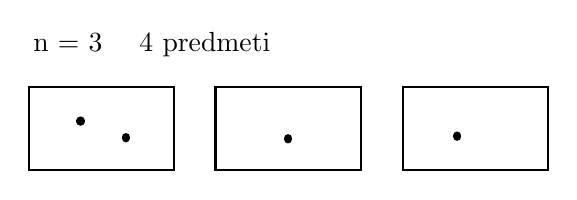
\begin{tikzpicture}[x=0.75pt,y=0.75pt,yscale=-1,xscale=1]
%uncomment if require: \path (0,300); %set diagram left start at 0, and has height of 300

%Shape: Rectangle [id:dp7407184316163662] 
\draw   (90.25,90.25) -- (160.25,90.25) -- (160.25,130.25) -- (90.25,130.25) -- cycle ;
%Shape: Rectangle [id:dp5723531652661165] 
\draw   (180.25,90.25) -- (250.25,90.25) -- (250.25,130.25) -- (180.25,130.25) -- cycle ;
%Shape: Rectangle [id:dp06732545223532949] 
\draw   (270.5,90.25) -- (340.5,90.25) -- (340.5,130.25) -- (270.5,130.25) -- cycle ;
%Shape: Free Drawing [id:dp5149127238979943] 
\draw  [line width=3] [line join = round][line cap = round] (115.25,106.76) .. controls (115.25,106.59) and (115.25,106.43) .. (115.25,106.26) ;
%Shape: Free Drawing [id:dp5804075845098335] 
\draw  [line width=3] [line join = round][line cap = round] (137,114.76) .. controls (137,114.59) and (137,114.43) .. (137,114.26) ;
%Shape: Free Drawing [id:dp5627736685120888] 
\draw  [line width=3] [line join = round][line cap = round] (215.25,115.26) .. controls (215.25,115.09) and (215.25,114.93) .. (215.25,114.76) ;
%Shape: Free Drawing [id:dp5538210827206191] 
\draw  [line width=3] [line join = round][line cap = round] (296.75,114.01) .. controls (296.75,113.84) and (296.75,113.68) .. (296.75,113.51) ;

% Text Node
\draw (91,62) node [anchor=north west][inner sep=0.75pt]   [align=left] {n = 3 \ \ \ 4 predmeti};


\end{tikzpicture}
    
\end{figure}


\subsubsection{Dokaz}
S protislovjem. Recimo, da je v vsaki škatli največ en predmet.
Potem zaključimo da je vseh predmetov največ $n$, kar je v protislovju s predpostavko, da imamo vsaj $n+1$ predmetov.


\subsubsection{Zgled}
\begin{enumerate}[label=\roman*.]
    \item Vsaki množici z več kot 12 osebami obstajata dve , ki imata rojstni dan v istem mescu. (škatle predstavljajo mesece)
    \item V vsaki množici z več kot 366 osebami obstajata dve, ki imata rojstni dan, na isti dan. (škatle predstavljajo dneve)
    \item Za vsako naravno število $n$ obstaja večkratnik tega števila katerega lahko zapišemo samo s pomočjo cifer 0 in 1.
    \begin{center}
        \begin{tabular}{c|l}
            $n$ &  \\  
            \hline
            1 & 1 \\
            \hline
            2 & 10 \\ 
            \hline
            3 & 111 \\
            \hline
            4 & 100 \\
            \hline
            6 & 1110
        \end{tabular}
    \end{center}
    Naj bo $n$ naravno število. Poglejmo si naslednje zaporedje naravnih števil:
    $$
    1, 11, 111, \dots, \underset{n}{\underbrace{111\ldots 1}}
    $$
    \begin{center}
        \begin{tabular}{r|c}
            $p$ & $p \text{ mod } 6$ \\  
            \hline
            1 & 1 \\
            \hline
            11 & 5 \\ 
            \hline
            111 & 3 \\
            \hline
            1111 & 1 \\
            \hline
            11111 & 5 \\
            \hline
            111111 & 3 \\
        \end{tabular}
    \end{center}
    Če je kakšno izmed njih deljivo z $n$ je problem rešen. V nasprotnem primeru da vsako izmed teh števil pri deljenju z $n$ enega od $n - 1$ možnih ostankov $1, \dots, n - 1$. \\
    Kar je v zaporedju $n$ števil, po Dirichletovom načelu obstajata dve števili v zaporedju, na primer:
    $$
    \underset{k}{\underbrace{11\ldots 1}} \text{ in } \underset{l}{\underbrace{11\ldots 1}}, \text{ } \text{ }\text{ }\text{ } k < l
    $$
    ki data isti ostanek pri deljenju z $n$. Potem pa je njuna razlika:
    $$
    \underset{l - k}{\underbrace{11\ldots 1}}\underset{k}{\underbrace{0 \ldots 0}}
    $$
    deljiva z $n$.
    \item V skupini dveh ali več ljudi lahko vedno najdemo dva, ki imata v tej skupini enako število prijateljev. (predpostavimo, da je relacija prijateljstva simetrična: $x$ je prijatelj z $y$ natanko tedaj, ko je $y$ prijatelj z $x$). Recimo, da skupino sestavlja $n$ ljudi: Razporedimo, ljudi v prostoru glede na to koliko prijateljev imajo.
    Število prostorov = številu ljudi (in ne moremo na začetku uporabiti Dirichletovega načela), vendar pa opazimo da je vsaj eden od prostorov vedno prazen, če prostor $n - 1$ ni prazen, potem obstaja oseba $x$, ki ima $n - 1$ prijateljev, torej je vsaka oseba prijatelj z osebo $x$ in zato ne obstaja oseba, ki ima 0 prijateljev.
    Torej je $n$ oseb razporejenih v $n-1$ prostorov. Po Dirichletovem načelu obstajata vsaj dve osebi, ki se nahajata v istem prostoru, in imata torej enako število prijateljev.
\end{enumerate}


\subsection{Izrek (posplošeno Dirichletovo načelo)}
Če $m$ predmetov razporedimo v $n$ škatel in velja da je:
$$
m > k \cdot n
$$
potem imamo vsaj v eni škatli vsaj $k + 1$ predmetov.
\begin{opomba}
    Neenakost je najboljša možna. \\
    Če je $m = k \cdot n$, lahko vsaka od $n$ škatel vsebuje natanko k objektov.
\end{opomba}


\subsubsection{Zgled}
\begin{enumerate}[label=\roman*.]
    \item 
    \begin{align*}
        \heartsuit \text{ }\text{ }\text{ } 1, \dots, 13 \\
        \diamondsuit \text{ }\text{ }\text{ } 1, \dots, 13 \\
        \clubsuit \text{ }\text{ }\text{ } 1, \dots, 13 \\
        \spadesuit \text{ }\text{ }\text{ } 1, \dots, 13 \\
    \end{align*}
    Najmanj koliko kart moramo izvleči iz standardnega kompleta 52 kart, da bodo med izvlečenimi kartami gotovo štiri karte iste barve (4 $\heartsuit$ ali 4 $\diamondsuit$ ali 4 $\clubsuit$ ali 4 $\spadesuit$)?
    \begin{align*}
        \text{predmeti = karte} \text{ }\text{ }\text{ } & k + 1 = 4 \\
        \text{škatle = barve} \text{ }\text{ }\text{ } & k = 3
    \end{align*}
    Predpostavimo da imamo 4 škatle, vsako rezerviramo z posamezno barvo. Ko karto izvlečemo, jo damo v pripadajočo škatlo. Iz posplošenega Drirchletovega načela vidimo, da je dovolj izvleči:
    $$
    13 \text{ }\text{ }\text{ } ( = 3 \cdot 4 + 1)
    $$
    kart, da bodo med izvlečenimi kartami gotovo štiri iste barve.
    \item V množici šestih oseb vedno obstajajo tri osebe ki se poznajo med sabo, ali pa obstajajo tri osebe, ki se ne poznajo med sabo.
    \begin{figure}[H]
    \centering



\tikzset{every picture/.style={line width=0.75pt}} %set default line width to 0.75pt        

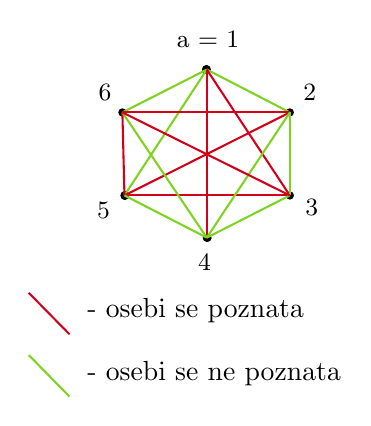
\begin{tikzpicture}[x=0.75pt,y=0.75pt,yscale=-1,xscale=1]
%uncomment if require: \path (0,300); %set diagram left start at 0, and has height of 300

%Shape: Free Drawing [id:dp32097770888647337] 
\draw  [line width=3] [line join = round][line cap = round] (159.67,39.17) .. controls (159.56,39.17) and (159.44,39.17) .. (159.33,39.17) ;
%Shape: Free Drawing [id:dp7115169153720922] 
\draw  [line width=3] [line join = round][line cap = round] (199.67,59.83) .. controls (199.67,59.83) and (199.67,59.83) .. (199.67,59.83) ;
%Shape: Free Drawing [id:dp7380766200951967] 
\draw  [line width=3] [line join = round][line cap = round] (199.67,99.83) .. controls (199.67,99.83) and (199.67,99.83) .. (199.67,99.83) ;
%Shape: Free Drawing [id:dp8120817520986101] 
\draw  [line width=3] [line join = round][line cap = round] (160,120.17) .. controls (159.89,120.17) and (159.78,120.17) .. (159.67,120.17) ;
%Shape: Free Drawing [id:dp9466386442036974] 
\draw  [line width=3] [line join = round][line cap = round] (120,99.83) .. controls (120.11,99.83) and (120.22,99.83) .. (120.33,99.83) ;
%Shape: Free Drawing [id:dp1225137644809009] 
\draw  [line width=3] [line join = round][line cap = round] (119,59.83) .. controls (119.44,59.83) and (119.44,59.83) .. (119,59.83) ;
%Straight Lines [id:da2840021976938738] 
\draw [color={rgb, 255:red, 126; green, 211; blue, 33 }  ,draw opacity=1 ]   (159.67,39.17) -- (199.67,59.83) ;
%Straight Lines [id:da6505289775895382] 
\draw [color={rgb, 255:red, 126; green, 211; blue, 33 }  ,draw opacity=1 ]   (159.67,39.17) -- (120,99.83) ;
%Straight Lines [id:da3333291940431733] 
\draw [color={rgb, 255:red, 126; green, 211; blue, 33 }  ,draw opacity=1 ]   (159.67,39.17) -- (119,59.83) ;
%Straight Lines [id:da931797594293039] 
\draw [color={rgb, 255:red, 208; green, 2; blue, 27 }  ,draw opacity=1 ]   (159.67,39.17) -- (199.67,99.83) ;
%Straight Lines [id:da3492860647128406] 
\draw [color={rgb, 255:red, 208; green, 2; blue, 27 }  ,draw opacity=1 ]   (159.67,39.17) -- (159.67,120.17) ;
%Straight Lines [id:da6299174165098118] 
\draw [color={rgb, 255:red, 208; green, 2; blue, 27 }  ,draw opacity=1 ]   (199.67,59.83) -- (119,59.83) ;
%Straight Lines [id:da6182573245467236] 
\draw [color={rgb, 255:red, 208; green, 2; blue, 27 }  ,draw opacity=1 ]   (199.67,59.83) -- (120,99.83) ;
%Straight Lines [id:da13979567508018587] 
\draw [color={rgb, 255:red, 208; green, 2; blue, 27 }  ,draw opacity=1 ]   (119,59.83) -- (120,99.83) ;
%Straight Lines [id:da24645412624051444] 
\draw [color={rgb, 255:red, 208; green, 2; blue, 27 }  ,draw opacity=1 ]   (199.67,99.83) -- (120,99.83) ;
%Straight Lines [id:da997567757393724] 
\draw [color={rgb, 255:red, 126; green, 211; blue, 33 }  ,draw opacity=1 ]   (199.67,59.83) -- (159.67,120.17) ;
%Straight Lines [id:da4087800300646556] 
\draw [color={rgb, 255:red, 126; green, 211; blue, 33 }  ,draw opacity=1 ]   (199.67,99.83) -- (159.67,120.17) ;
%Straight Lines [id:da8300135504005863] 
\draw [color={rgb, 255:red, 126; green, 211; blue, 33 }  ,draw opacity=1 ]   (120,99.83) -- (159.67,120.17) ;
%Straight Lines [id:da1645578346196419] 
\draw [color={rgb, 255:red, 126; green, 211; blue, 33 }  ,draw opacity=1 ]   (119,59.83) -- (159.67,120.17) ;
%Straight Lines [id:da3585377298938379] 
\draw [color={rgb, 255:red, 126; green, 211; blue, 33 }  ,draw opacity=1 ]   (199.67,59.83) -- (199.67,99.83) ;
%Straight Lines [id:da6152415716874657] 
\draw [color={rgb, 255:red, 208; green, 2; blue, 27 }  ,draw opacity=1 ]   (199.67,99.83) -- (119,59.83) ;
%Straight Lines [id:da920189752176505] 
\draw [color={rgb, 255:red, 208; green, 2; blue, 27 }  ,draw opacity=1 ]   (93.53,166.73) -- (73.87,146.73) ;
%Straight Lines [id:da6993823771422543] 
\draw [color={rgb, 255:red, 126; green, 211; blue, 33 }  ,draw opacity=1 ]   (93.53,196.73) -- (73.87,176.73) ;

% Text Node
\draw (143.67,19.5) node [anchor=north west][inner sep=0.75pt]  [font=\small] [align=left] {a = 1};
% Text Node
\draw (105.33,101.5) node [anchor=north west][inner sep=0.75pt]  [font=\small] [align=left] {5};
% Text Node
\draw (106,44.83) node [anchor=north west][inner sep=0.75pt]  [font=\small] [align=left] {6};
% Text Node
\draw (154,126.83) node [anchor=north west][inner sep=0.75pt]  [font=\small] [align=left] {4};
% Text Node
\draw (205.67,100.17) node [anchor=north west][inner sep=0.75pt]  [font=\small] [align=left] {3};
% Text Node
\draw (204.67,44.83) node [anchor=north west][inner sep=0.75pt]  [font=\small] [align=left] {2};
% Text Node
\draw (100.67,148.07) node [anchor=north west][inner sep=0.75pt]   [align=left] {\mbox{-} osebi se poznata};
% Text Node
\draw (100.67,178.4) node [anchor=north west][inner sep=0.75pt]   [align=left] {\mbox{-} osebi se ne poznata};


\end{tikzpicture}

\end{figure}
    Naj bo $a$ poljubno izbrana oseba iz množice. Razdelimo naslednjih 5 oseb v dva prostora.
    \begin{figure}[H]
    \centering
    


\tikzset{every picture/.style={line width=0.75pt}} %set default line width to 0.75pt        

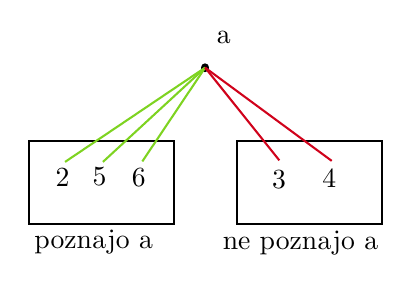
\begin{tikzpicture}[x=0.75pt,y=0.75pt,yscale=-1,xscale=1]
%uncomment if require: \path (0,300); %set diagram left start at 0, and has height of 300

%Shape: Rectangle [id:dp9910313861609417] 
\draw   (80,70.25) -- (150,70.25) -- (150,110.25) -- (80,110.25) -- cycle ;
%Shape: Rectangle [id:dp6524445408103099] 
\draw   (180.25,70) -- (250.25,70) -- (250.25,110) -- (180.25,110) -- cycle ;
%Shape: Free Drawing [id:dp9635620821980186] 
\draw  [line width=3] [line join = round][line cap = round] (165,34.93) .. controls (165,34.84) and (165,34.76) .. (165,34.68) ;
%Straight Lines [id:da8845189038102581] 
\draw [color={rgb, 255:red, 126; green, 211; blue, 33 }  ,draw opacity=1 ]   (165,34.76) -- (97.5,80.18) ;
%Straight Lines [id:da8889347170043365] 
\draw [color={rgb, 255:red, 126; green, 211; blue, 33 }  ,draw opacity=1 ]   (165,34.76) -- (115.75,80.18) ;
%Straight Lines [id:da7198798826573838] 
\draw [color={rgb, 255:red, 126; green, 211; blue, 33 }  ,draw opacity=1 ]   (165,34.76) -- (134.75,79.93) ;
%Straight Lines [id:da7212265299933625] 
\draw [color={rgb, 255:red, 208; green, 2; blue, 27 }  ,draw opacity=1 ]   (165,34.76) -- (200.75,79.43) ;
%Straight Lines [id:da854036126090751] 
\draw [color={rgb, 255:red, 208; green, 2; blue, 27 }  ,draw opacity=1 ]   (165,34.76) -- (226,79.68) ;

% Text Node
\draw (169,16) node [anchor=north west][inner sep=0.75pt]   [align=left] {a};
% Text Node
\draw (91.5,82) node [anchor=north west][inner sep=0.75pt]   [align=left] {2};
% Text Node
\draw (109.25,81.5) node [anchor=north west][inner sep=0.75pt]   [align=left] {5};
% Text Node
\draw (128.25,82) node [anchor=north west][inner sep=0.75pt]   [align=left] {6};
% Text Node
\draw (195.75,82.75) node [anchor=north west][inner sep=0.75pt]   [align=left] {3};
% Text Node
\draw (220,82.5) node [anchor=north west][inner sep=0.75pt]   [align=left] {4};
% Text Node
\draw (81.25,111.5) node [anchor=north west][inner sep=0.75pt]   [align=left] {poznajo a};
% Text Node
\draw (172,111.75) node [anchor=north west][inner sep=0.75pt]   [align=left] {ne poznajo a};


\end{tikzpicture}
\end{figure}
    Ker je $5 > 2 \cdot 2$, po Dirichletovem načelu obstaja en prostor z vsaj 3 osebami.
    \begin{figure}[H]
    \centering




    \tikzset{every picture/.style={line width=0.75pt}} %set default line width to 0.75pt        

    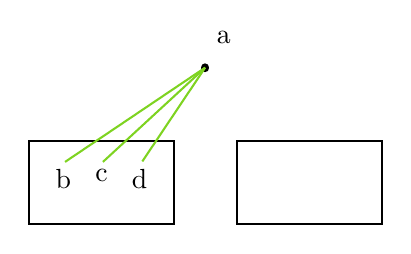
\begin{tikzpicture}[x=0.75pt,y=0.75pt,yscale=-1,xscale=1]
    %uncomment if require: \path (0,300); %set diagram left start at 0, and has height of 300
    
    %Shape: Rectangle [id:dp05929262611884156] 
    \draw   (80,70.25) -- (150,70.25) -- (150,110.25) -- (80,110.25) -- cycle ;
    %Shape: Rectangle [id:dp4641637777411629] 
    \draw   (180.25,70) -- (250.25,70) -- (250.25,110) -- (180.25,110) -- cycle ;
    %Shape: Free Drawing [id:dp486851933115376] 
    \draw  [line width=3] [line join = round][line cap = round] (165,34.93) .. controls (165,34.84) and (165,34.76) .. (165,34.68) ;
    %Straight Lines [id:da7642309413451847] 
    \draw [color={rgb, 255:red, 126; green, 211; blue, 33 }  ,draw opacity=1 ]   (165,34.76) -- (97.5,80.18) ;
    %Straight Lines [id:da4565983768062105] 
    \draw [color={rgb, 255:red, 126; green, 211; blue, 33 }  ,draw opacity=1 ]   (165,34.76) -- (115.75,80.18) ;
    %Straight Lines [id:da3386816838548048] 
    \draw [color={rgb, 255:red, 126; green, 211; blue, 33 }  ,draw opacity=1 ]   (165,34.76) -- (134.75,79.93) ;
    
    
    % Text Node
    \draw (169,16) node [anchor=north west][inner sep=0.75pt]   [align=left] {a};
    % Text Node
    \draw (91.5,82) node [anchor=north west][inner sep=0.75pt]   [align=left] {b};
    % Text Node
    \draw (110.58,82.5) node [anchor=north west][inner sep=0.75pt]   [align=left] {c};
    % Text Node
    \draw (128.25,82) node [anchor=north west][inner sep=0.75pt]   [align=left] {d};
    
    
    \end{tikzpicture}
    
\end{figure}
    Predpostavimo najprej, da so v prvem prostoru osebe $b, c, d$. Če se kakšni dve izmed teh oseb poznata med seboj, na primer $b$ in $c$ potem je $\{a, b, c\}$ podmnožica teh oseb ki se med seboj poznajo. V nasprotnem primeru pa se nobeni dve osebi iz podmnožice $\{b, c, d\}$ ne poznata. Primer, ko se ti osebi nahajajo v drugem prostoru, obravnavamo podobno.
\end{enumerate}
